\documentclass{article}
\usepackage[utf8]{inputenc}
\usepackage{geometry}
\geometry{
	a4paper,
	total={170mm,257mm},
	left=20mm,
	top=20mm,
}
\usepackage{graphicx}
\usepackage{titling}
\usepackage[american,RPvoltages]{circuiTikz}
\usepackage{tikz, tikz-cd}
\usepackage{pgfplots}
\usepackage{siunitx}
\usepackage{float}
\usepackage{enumitem}
\usepackage{amsmath,amsfonts,stmaryrd,amssymb} % Math packages
\usepackage{schemabloc}
\usetikzlibrary{circuits}
\usetikzlibrary{positioning}
\title{Osciladores}
\author{Rodrigo Castillejos}
\date{July 2024}

\usepackage{fancyhdr}
\fancypagestyle{plain}{%  the preset of fancyhdr 
	\fancyhf{} % clear all header and footer fields
	\fancyfoot[L]{\thedate}
	\fancyhead[L]{Osciladores}
	\fancyhead[R]{\theauthor}
}
\makeatletter
\def\@maketitle{%
	\newpage
	\null
	\vskip 1em%
	\begin{center}%
		\let \footnote \thanks
		{\LARGE \@title \par}%
		\vskip 1em%
		%{\large \@date}%
	\end{center}%
	\par
	\vskip 1em}
\makeatother

\usepackage{lipsum}  
\usepackage{cmbright}

\begin{document}
	
	\maketitle
	
	\noindent\begin{tabular}{@{}ll}
		Author & \theauthor\\
		Chapter &  Basic Circuit Analysis\\
		Problem & 2.68
	\end{tabular}
	
	\section*{Resumen}
En el diseño de sistemas electrónicos, frecuentemente surge la necesidad de generar señales con formas de ondas prescritas o estándar, por ejemplo, formas de onda senoidales, cuadradas, triangulares o de pulso. Los osciladores suelen encontrarse, por citas algunos ejemplos, en los microprocesadores que utilizan el generador de reloj (fabricado en el mismo chip utilizando osciladores de anillo con frecuencias en el rango de los GHz), el generador de la forma de onda portadora en los transceptores inalámbricos (en el rango de centenas de GHz), el oscilador en un reloj electrónico (utilizando cristales de cuarzo con una frecuencia de $2^{15}$ Hz) y los generadores de funciones de frecuencia variable en los equipos de laboratorio (utilizando circuitos discretos con frecuencia en el rango de los Hz a los MHz). \\

\noindent Hay dos técnicas utilizadas para la generación de senoides. La primera técnica emplea un \textbf{lazo de realimentación positiva} el cual consiste de una \textbf{red de frecuencia selectiva} a base de un circuito RC o LC. Mientras que la frecuencia de la onda senoidal generada la determina la red de frecuencia selectiva, la amplitud se establece empleando mecanismos no lineales, implementadas o bien con un circuito separado las no linealidades del dispositivo amplificador mismo. A pesar de lo antes mencionado, estos circuitos que generan ondas senoidales utilizando el efecto de la resonancia son conocidos como \textbf{osciladores lineales}. Este nombre los distingue de los circuitos que generan ondas senoidales a través del segundo enfoque. En estos circuitos la senoide se obtiene a partir de una señal triangular.\\

\noindent En general, los circuitos que generan formas de onda cuadradas, triangulares o de pulso son llamados \textbf{osciladores no lineales} o \textbf{generador de funciones} y emplean bloques de circuitos conocidos como \textbf{multivibradores}. Existen tres tipos de multivibradores: el \textbf{biestable}, el \textbf{astable} y el \textbf{monoestable}

\section{Principios básicos de los osciladores senoidales}
A pesar del nombre de \textit{oscilador lineal}, es común emplear alguna técnica no lineal para proporcionar un control de amplitud sobre la onda senoidal de salida. De hecho, todos los osciladores son escencialmente circuitos no lineales. Esto complica la tarea de análisis y diseño de los osciladores ya que no se puede emplear los métodos de transformación en el plano $s$ directamente 

\subsection{El lazo de realimentación - condiciones de oscilación}
La estructura básica de un oscilador senoidal consiste de un amplificador y una red de frecuencia selectiva conectada en un \textbf{lazo de realimentación positiva} como el que se muestra en el diagrama de bloques de la figura 1. A pesar de que en realidad no hay una señal de entrada presente en un circuito oscilador, en el diagrama de bloques se incluye una señal de entrada para ayudar a explicar el principio de operación. Es importante mencionar que a diferencia del lazo de realimentación negativo, aquí la señal de realimentación $v_f$ es sumada con un signo \textit{positivo}.

\begin{figure}[H]
	\centering
	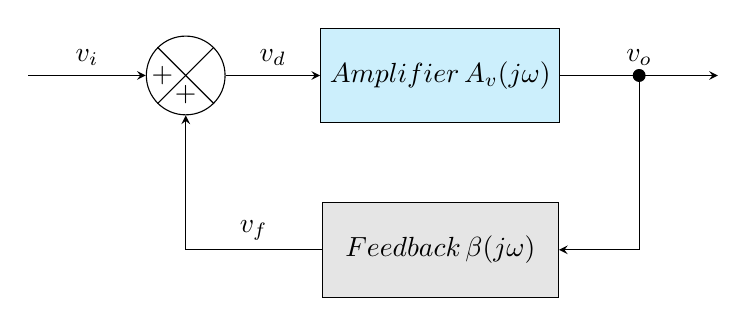
\begin{tikzpicture}
		%Sum block
		\node[draw, circle, minimum size=1cm] (sum) at (0,0){};
		\draw (sum.north east) -- (sum.south west);
		\draw (sum.north west) -- (sum.south east);
		\node[left = 1pt] at (sum.center){$+$};
		\node[below] at (sum.center){$+$};
		
		%First Block
		\node[draw,
		      fill=cyan!20,
		      minimum width = 3cm,
		      minimum height = 1.2cm,
		      right= 1.2cm of sum] (Block1){$Amplifier \, A_v(j\omega)$};
		
		%Feedback Block
		\node[draw,
		      fill=gray!20,
		      minimum width = 3cm,
		      minimum height = 1.2cm,
		      below = 1cm of Block1] (Feedback){$Feedback \, \beta(j \omega)$};
		      
		\draw[-stealth](sum.east) -- (Block1.west) node[midway, above]{$v_d$};
		\draw[-stealth](Block1.east) -- ++ (2,0) node[midway](output){} node[midway, above]{$v_o$};
		\draw[-stealth](output.center) |- (Feedback.east);
		\node[draw, circle, fill=black, inner sep=0pt, minimum size=0.15cm] (mynode) at (output.center){};
		\draw[-stealth](Feedback.west)  -| (sum.south) node[near start, above]{$v_f$};
		\draw[-stealth] (-2,0) -- (sum.west) node[midway, above]{$v_i$};
	\end{tikzpicture}
\caption{}	
\label{fig:figura1}
\end{figure}

La ganancia del amplificador $A_v(j \omega)$ es también llamada ganancia en lazo abierto dado que es la ganancia entre $v_o$ y $v_i$ cuando $v_f=0$ (es decir, cuando el camino a través de $\beta (j\omega)$ es desconectado por completo). La ganancia del amplificador es, en general, una cantidad compleja. De la figura 1 podemos escribir:

\begin{align}
	v_o = A_v (j \omega)v_d  \\
	v_f = \beta (j \omega) v_o
\end{align}

Y

\begin{align}
	v_d = v_i + v_f
\end{align}

Así, de las ecuaciones (1) a (3) podemos calcular la ganancia de lazo cerrado $A_{vf}(j \omega)$


\begin{align}
	A_{vf}(j \omega) = \frac{v_o}{v_i} = \frac{A_v(j\omega)}{1 - \beta(j \omega) A_v (j \omega)}
\end{align}

Nótese el signo negativo en el denominador. Para que las oscilaciones ocurran, no debe existir ninguna señal de entrada aplicada, Con $v_i = 0$, un $v_o$ finito sólo es posible en (4) cuando el denominador es cero, esto es cuando:

\begin{align}
	1 - \beta (j\omega)A_v (j\omega) = 0 \nonumber
\end{align}

o 

\begin{align}
	\beta (j\omega)A_v (j\omega) = 1
\end{align}

La ecuación expresa el hecho de que para que las oscilaciones ocurran la ganancia de lazo debe ser unitaria. Esta relación es conocida como el criterio de Barkhausen.

Sea

\begin{align}
	\beta (j \omega) = \beta_r(\omega) + j\beta_i (\omega)
\end{align}

Donde $\beta_r(\omega)$ y $\beta_i(\omega)$ son la parte real e imaginaria de $\beta(j\omega)$, entonces podemos expresar (5) en la forma

\begin{align}
	\beta_r(\omega)A_{v0} + j\beta_i(\omega)A_{v0} = 1\nonumber
\end{align}

\subsection{Criterio de oscilación}
En una frecuencia específica $f_0$ la ganancia de lazo $A \beta$ será igual a la unidad, eso significaría que en (4) $A_{vf}$ sería infinita. Esto es, a esta frecuencia el circuito tendrá una salida finita para una señal de entrada nula o igual a cero. Tal circuito es por definición un oscilador. Por lo tanto, la condición para que el lazo de realimentación de la figura 1 proporcione oscilaciones senoidales de frecuencia $w_0$ es

\begin{align}
	L(j\omega_0) = A_v(j \omega_0)\beta(j\omega_0) = 1
\end{align}

\section*{Oscilador de Puente de Wien}
El oscilador de puente de Wien es de amplio uso en la generación de senoides en la gama de frecuencias inferior a $\qty{1}{\mega \hertz}$.
Como se observa en la figura 2, este oscilador consta en esencia de un amplificador no inversor con dos trayectorias de realimentación : la trayectoria de realimentación positiva en la entrada no inversora crea oscilaciones, mientras que la trayectoria de realimentación negativa en la entrada inversora ayuda a controlar la ganancia.

Podemos calcular la ganancia $A_v(j \omega)$ empleando la LCK en el nodo inversor como sigue:

\begin{align}
	I_{RG} &= I_{RF} \nonumber \\
	\frac{-V_2}{R_G} &= \frac{V_2 - V_o}{R_F} \nonumber \\
	\frac{V_o}{R_F} &= \left[ \frac{1}{R_F} + \frac{1}{R_G} \right] V_2  \nonumber \\
	\frac{V_o}{R_F} &= \left[ \frac{R_F + R_G}{R_F R_G} \right] V_2  \nonumber
\end{align}

	\begin{figure}[H]
		\centering
	\begin{tikzpicture}[scale=0.8]
		\ctikzset{bipoles/thickness=4}
		\ctikzset{monopoles/vcc/arrow={Stealth[width=6pt,length=9pt]}}
		\ctikzset{monopoles/vee/arrow={Stealth[width=6pt,length=9pt]}}
		\draw (0,0) node[op amp, anchor=+](OA){};
		\draw (OA.-) to[short] ++(-2,0) coordinate (in1)
		      to[short] ++(0,2) coordinate (p1);
		\draw (p1) to[R, l=$R_F$] (p1 -| OA.out) -- (OA.out);
		\draw (in1) to[R, *-, l_=$R_G$] ++ (-3,0)
		      to[short] ++(0,-0.5) node[ground]{};
		\draw (OA.+) to[short] ++(-2,0)
		      to[short] ++(0,-2) coordinate (p2);
		\draw (p2) to[R, l=$R_1$] ++(3,0) to[cC, l=$C_1$] (p2 -| OA.out) -- (OA.out);
		\draw (OA.out) to[short, *-o] ++(2,0) coordinate(out1);
		\draw (p2) to[R, *-, l= $R_2$] ++(0,-3) node[ground]{};
		\draw (p2) to[short] ++(-2,0) 
		      to[cC, l=$C_2$, v=$V_2$] ++(0,-3)node[ground]{};
		\draw (out1) to[open, -o, v=$V_o$] ++(0,-2.5) node[ground]{};
		\draw[<-] (4,3) -- (5,3.5);
		\draw node[above] at (5,4){$Trayectoria \, de \, retroalimentacion$};
		\draw node[above] at (5,3.5){$negativa \, para \, controlar\, la \, ganancia$};
		\draw[<-] (0.2,-3) -- (0.8,-3.5);
		\draw node[above] at (3,-4.5){$Trayectoria \, de \, retroalimentacion$};
		\draw node[above] at (3,-5){$positiva \, para \, crear \, oscilaciones$};
	\end{tikzpicture}
	\caption{}	
	\label{fig:figura2}
\end{figure}

\begin{align}
	V_o = \left[ \frac{R_F + R_G}{R_G} \right]V_2 \nonumber
\end{align}

Por lo tanto

\begin{align}
	A_v(j \omega) = A_{v0} = \frac{V_o}{V_2} = 1 + \frac{R_F}{R_G}
\end{align}

El voltaje en $V_2$ está dado por 

\begin{align}
	V_2 =  \frac{Z_p}{Z_s + Z_p}V_o
\end{align}

Donde

\begin{align}
	Z_p =  R_2 \Large{\parallel}  {\frac{1}{j \omega C2}}  = \frac{R_2}{1 + j \omega R_2 C_2}
\end{align}


Y

\begin{align}
	Z_s = R_1 + \frac{1}{j \omega C_1} = R_1 - \frac{j}{\omega C_1}
\end{align}

Por lo tanto

\begin{align}
	V_2  &= \frac{ \frac{R_2}{1 + j \omega R_2 C_2} }{ R_1 - \frac{j}{\omega C_1} + \frac{R_2}{1 + j \omega R_2 C_2} }V_o \nonumber \\
	&= \frac{1}{ \left( R_1 - \frac{j}{\omega C_1} \right) \left( \frac{1 + j \omega R_2C_2}{R_2} \right)  + 1}V_o \nonumber
\end{align}

En la mayoría de las aplicaciones prácticas $R_1 = R_2 = R$ y $C_1 = C_2 = C$, por lo tanto

\begin{align}
	V_2 &= \frac{1}{ \left( R - \frac{j}{\omega C} \right) \left( \frac{1 + j \omega RC}{R} \right) + 1 }V_o \nonumber \\
        &= \frac{1}{ \left( \frac{\omega RC - j}{\omega C} \right) \left( \frac{1 + j\omega RC}{R}  \right) +1 }V_o \nonumber\\
        &= \frac{1}{ \frac{ (\omega RC - j)(1 + j\omega RC) }{\omega RC} +1 }V_o \nonumber \\
        &= \frac{1}{ \left( \frac{ \omega RC + j\omega^2 R^2C^2 - j + \omega RC }{\omega RC} \right) + 1 }V_o \nonumber \\
        &= \frac{1}{ \frac{ \omega RC + j \omega^2 R^2C^2 + \omega RC + \omega RC - j }{\omega RC} }V_o \nonumber
\end{align}

Así, la razón de realimentación $\beta (j\omega)$ puede escribirse como

\begin{align}
	\beta (j \omega) = \frac{V_2}{V_o} = \frac{1}{3 + j\left( \omega RC - \frac{1}{\omega RC} \right)}
\end{align}

De las ecuaciones (7) y (11) la ganancia de lazo es

\begin{align}
	\beta (j \omega) A_{v0} = \frac{1}{3 + j \left( \omega RC - \frac{1}{\omega RC} \right)} \left( 1 +  \frac{R_F}{R_G} \right)
\end{align}

Para que se logren dar las oscilaciones la ganancia de lazo debe ser unitaria, esto es, la parte imaginaria de $\beta (j \omega)$ debe ser cero. Si igualamos el denominador de (11) a cero obtenemos

\begin{align}
	\omega RC - \frac{1}{\omega RC} = 0 \Rightarrow \omega = \omega_0 = \frac{1}{RC} \nonumber
\end{align}

O

\begin{align}
 \omega_0 = \frac{1}{RC}  \Rightarrow	f_0 = \frac{1}{2 \pi RC}
\end{align}

La sustitución de (13) en (11) produce 

\begin{align}
	\beta (j \omega) = \frac{V_2}{V_o} = \frac{1}{3 + j(\frac{1}{ RC} RC) - \frac{RC}{RC}} = \frac{1}{3}
\end{align}

Por lo tanto, la condición de ganancia es

\begin{align}
	A_{v0} = \frac{1}{\beta_r(\omega_0)} = 3
\end{align}

De la ecuación (8) obtenemos

\begin{align}
	\frac{V_o}{V_2} = 1 + \frac{R_F}{R_G} = 3
\end{align}

O sea

\begin{align}
	R_F = 2R_G
\end{align}

\subsection*{Control de amplitud no lineal}
Los circuitos limitadores se usan frecuentemente para el control de amplitud en osciladores con amplificadores operacionales, así como en una gran variedad de otras aplicaciones.


\end{document}